\section{EXPERIMENTAL RESULTS}

\begin{figure}
\centering
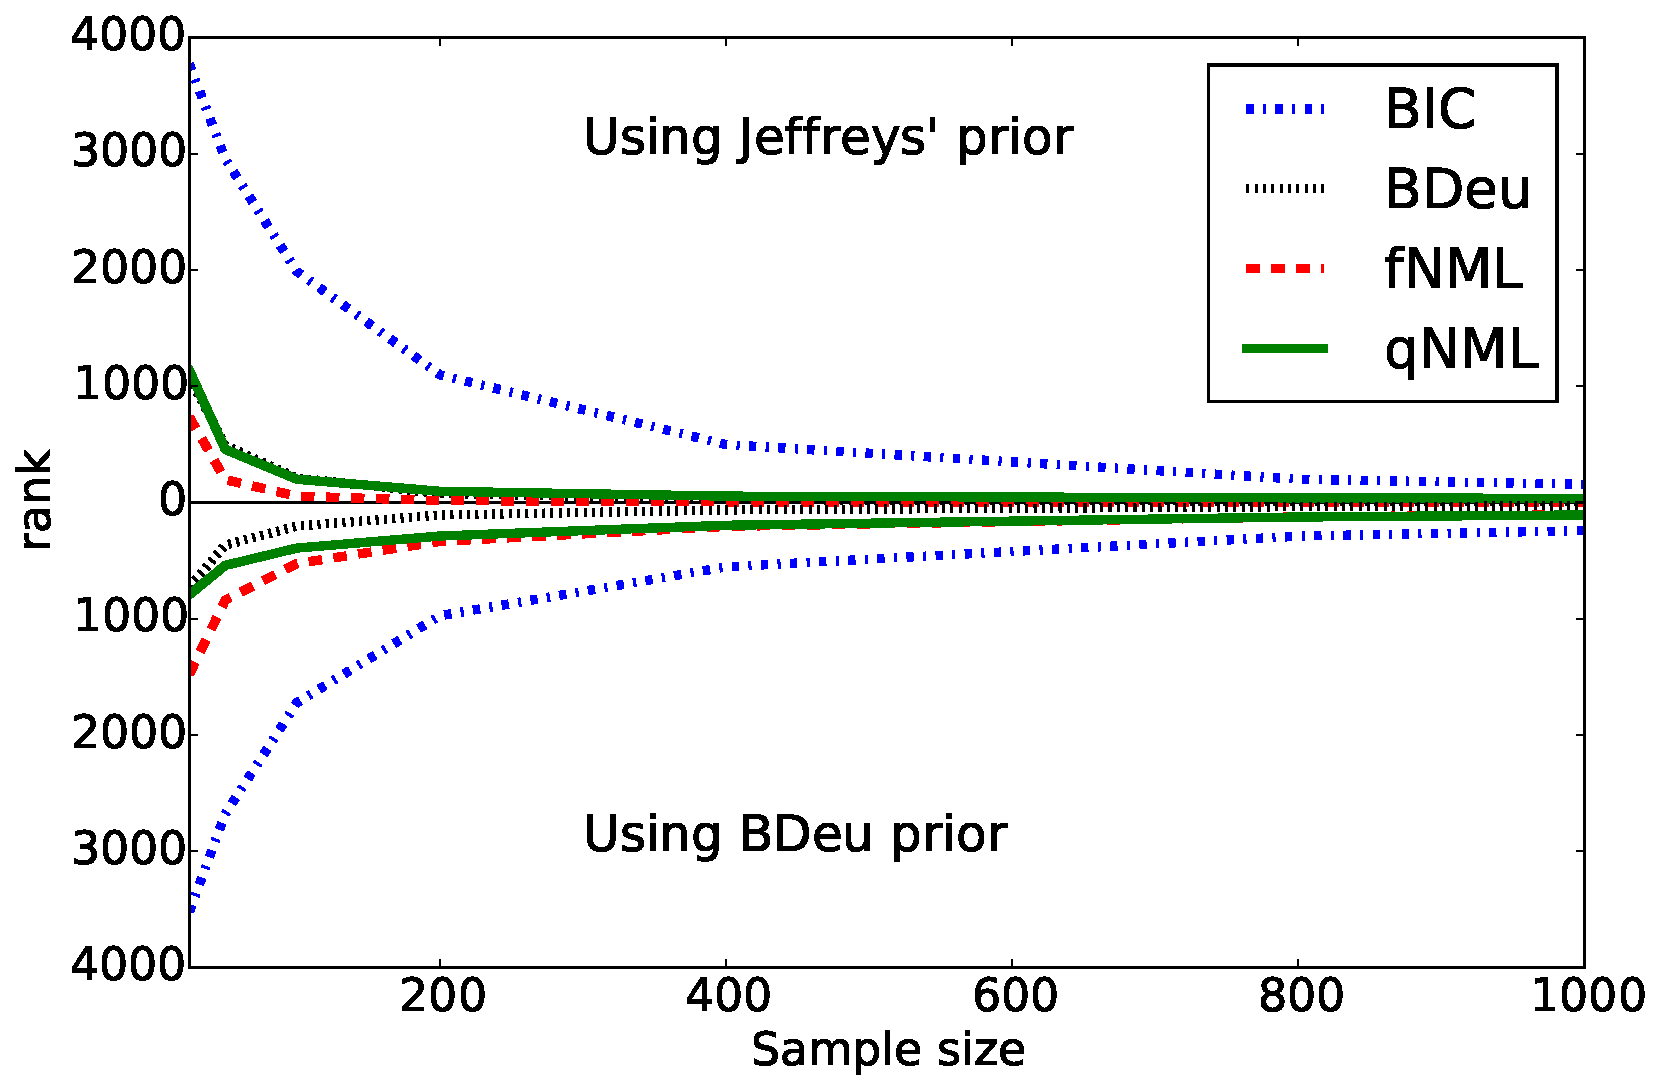
\includegraphics[width=8cm,height=5cm]{qNML_images/art4_mean.pdf}
\caption{Finding generating models of 4 arcs.}
\label{fig:4arcs}
\end{figure}

\begin{figure}
\centering
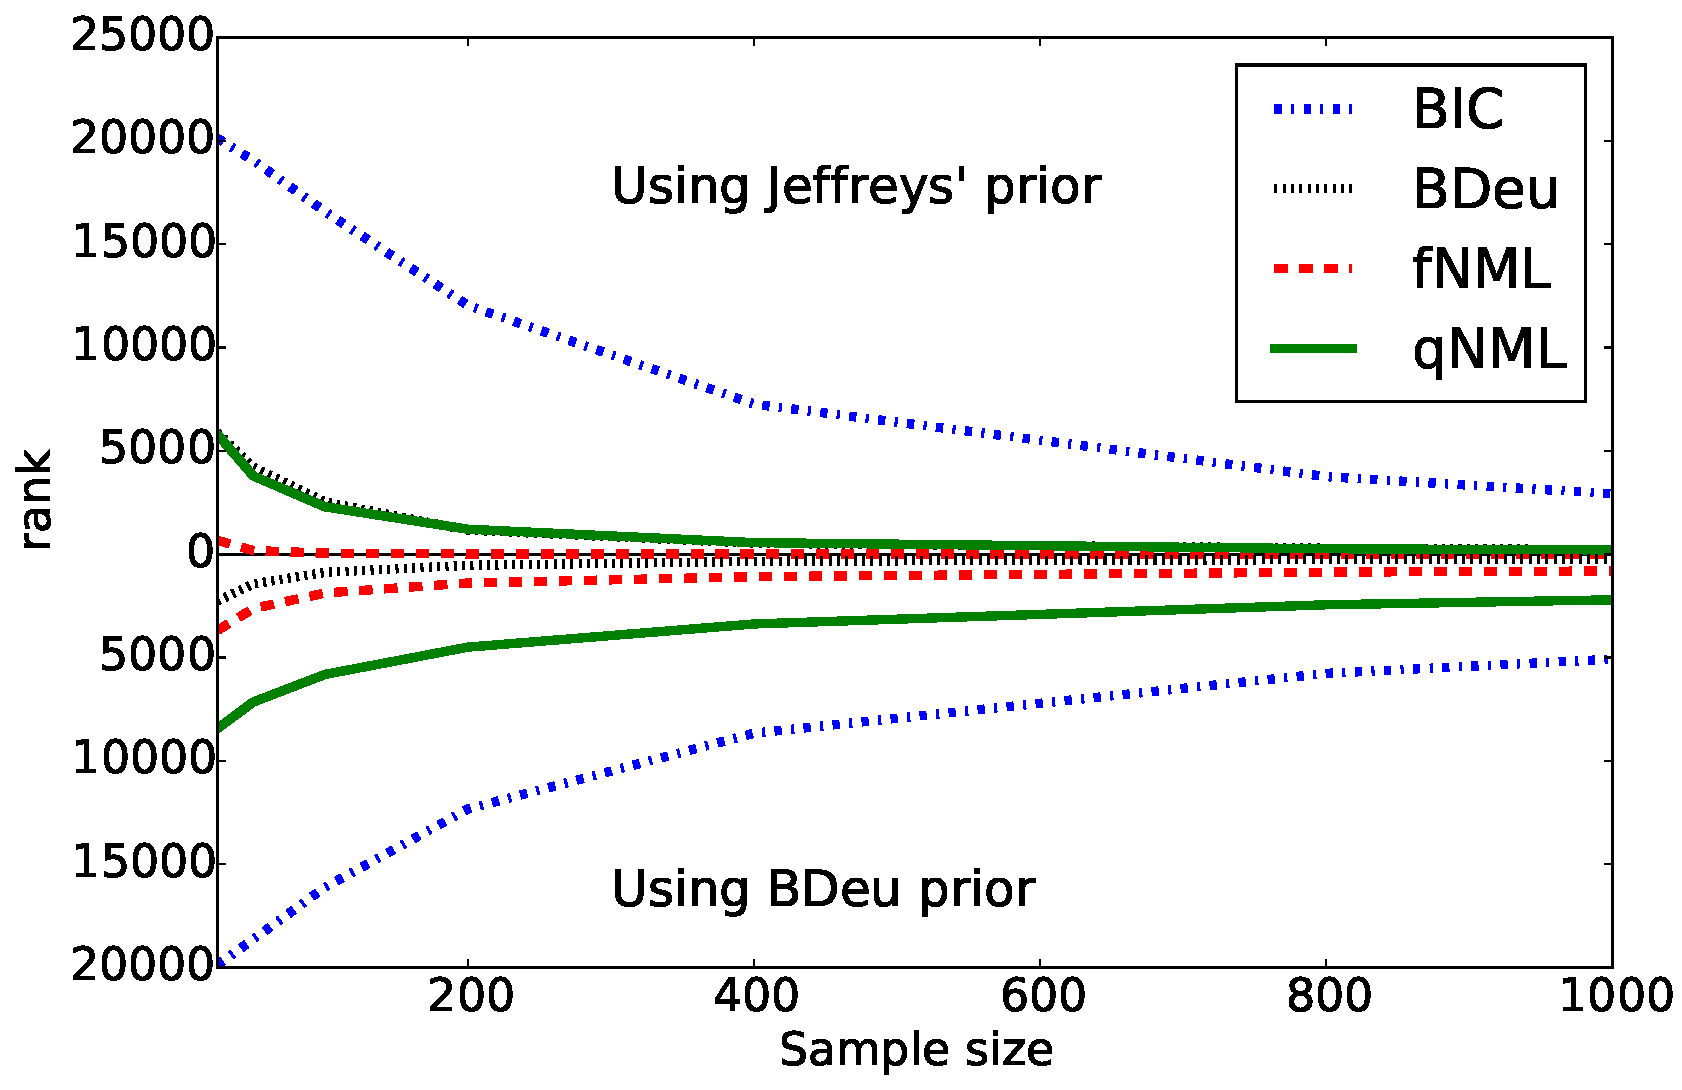
\includegraphics[width=8cm,height=5cm]{qNML_images/art7_mean.pdf}
\caption{Finding generating models of 7 arcs.}
\label{fig:4arcs}
\end{figure}

We empirically compare the capacity of qNML to that of BIC, BDeu and
fNML in identifying the data generating structures, and producing
models that are predictive and parsimonious.  It seems that none of
the criteria uniformly outperform the others in all these desirable
aspects of model selection criteria.

\subsection{FINDING GENERATING STRUCTURE}

We first compare the ability of the different scoring criteria to
discover the structure that generated the data. For this purpose we
create 100 random 5-node Bayesian network structures with 4
edges and another 100 structures with 7 edges.  The variables were
randomly assigned to have 2 -- 4 values ($r_i \in \{2, 3, 4\}$). For
each network, we generated parameters by two different schemes. The
first scheme exactly matched the assumptions of the BDeu score with
$\alpha = 1$, i.e., the parameters were distributed by $\theta_{ij}
\sim Dir(\frac{1}{r_iq_i},\ldots,\frac{1}{r_iq_i})$. The other scheme
was to generate the parameters independently from a Dirichlet
distribution $\theta_{ij} \sim Dir(\frac{1}{2},\ldots, \frac{1}{2})$
that is the Jeffreys' prior for the multinomial model. This distribution
was selected instead of the uniform distribution in order to make the
generating structure more identifiable.  For each network (structure +
parameters), we generated 100 data sets of 1000 data vectors, and
studied how different scoring criteria ranked the structure of the
generating network among all the 5-node networks as a function of
(sub)sample size.



Not surprisingly, the results indicate that when the parameter generation
mechanism matches the assumptions of the BDeu-score, BDeu usually
also ranks the generating structure higher than the other scores
(Figure X).  On the other hand, when the parameters are drawn from the
Jeffreys' prior, the fNML score appears to rank the generating structure
highest. This too is not surprising, since the NML distribution for
multinomial data is known to closely match the marginal distribution of
the data when the Jefrreys' prior is used.

The underfitting tendency of BIC can also be clearly detected both for
relatively sparse networks (4 arcs) and for dense ones (7 arcs). The
ranking ability the qNML criterion appears to be between fNML and BDeu
in 3 out of 4 settings which is good considering that one of these
criteria is always the winner. For the dense networks with BDeu prior,
qNML appears to perform worse than BDeu and fNML but still much
better than BIC.

\subsection{PREDICTION AND PARSIMONY}

To empirically compare the model selection criteria we took 20 UCI
data sets~\cite{Lichman:2013} and ran 1000 train and test experiments
for all of them. In each experiment, random 10\% of the original
dataset was selected as training data and the rest 90\% as test data.
The training was conducted using a dynamic programming based exact structure
learning~\cite{cosco.uai06} which limited the number $n$ of variables
to less than 20.

When predicting with structures learned by the BDeu score, we used the
Bayesian expected parameter values $\theta_{ijk} \propto
N_{ijk}+\frac{1}{r_iq_i}$.  In the spirit of keeping the scores
hyperparameter free, for structures learned by the other model
selection criteria, we used the predictive conditional NML
parametrization $\theta_{ijk}\propto e(n_{ijk})(n_{ijk}+1)$, where
$e(n)=(\frac{n+1}{n})^n$ as suggested in~\cite{Riss07b}.

\begin{figure}
\centering
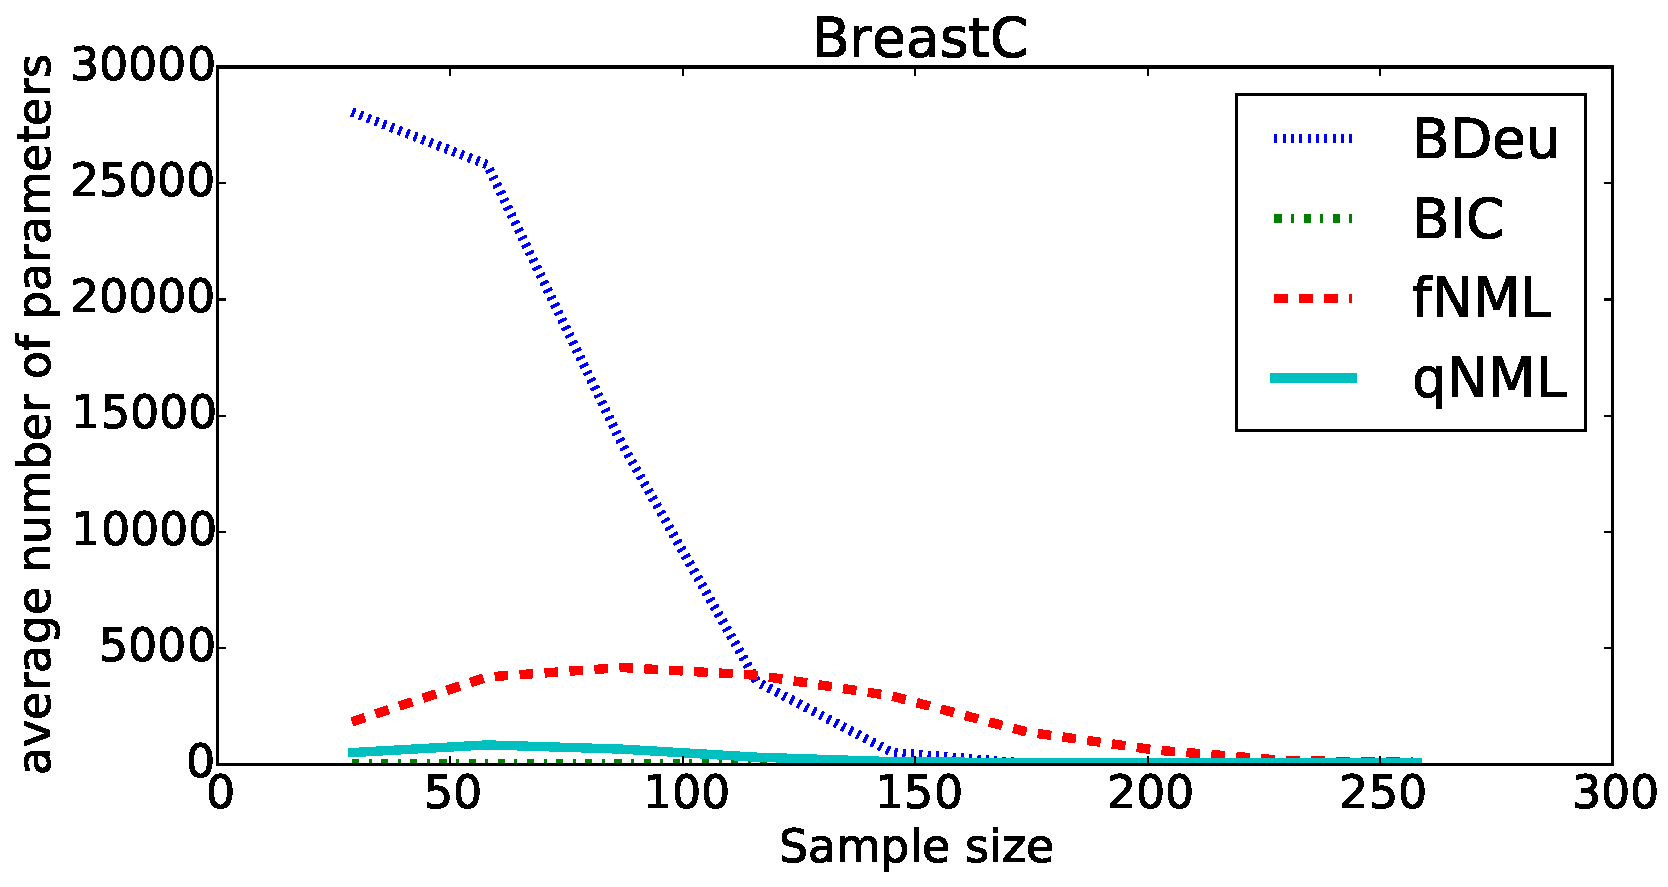
\includegraphics[width=8cm,height=5cm]{qNML_images/breast_cancer_npmean.pdf}
\caption{Number of parameters in a breast cancer model as a function
  of sample size for different model selection criteria.}
\label{fig:bcnpmean}
\end{figure}

\begin{table}
\caption{Predictive log losses for small sample sizes for different model selection criteria in 20 different datasets.}
\label{tbl:preds}
\begin{center}
 \begin{tabular}{crrrrr}
    Data &     N &              BDeu &               BIC &               fNML &               qNML \\
\midrule
    Iris &    15 &     \textit{3.61} &              3.56 &   \underline{3.50} &      \textbf{3.47} \\
 PostOpe &    18 &    \textit{10.52} &     \textbf{7.45} &   \underline{8.35} &               8.39 \\
   Ecoli &    34 &     \textit{6.27} &              6.16 &      \textbf{5.56} &   \underline{5.63} \\
   Liver &    35 &     \textit{4.22} &     \textbf{4.01} &               4.10 &   \underline{4.03} \\
    Wine &    36 &    \textit{16.41} &    \textbf{11.27} &              12.07 &  \underline{11.86} \\
   Glass &    44 &     \textit{7.48} &              6.65 &      \textbf{6.37} &   \underline{6.43} \\
 Thyroid &    44 &              2.92 &     \textit{2.93} &      \textbf{2.81} &   \underline{2.83} \\
 HeartSt &    54 &    \textit{14.37} &    \textbf{10.96} &              11.98 &  \underline{11.65} \\
 BreastC &    58 &    \textit{11.21} &     \textbf{9.94} &  \underline{10.34} &              10.37 \\
 HeartHu &    60 &     \textit{9.21} &     \textbf{8.38} &               8.80 &   \underline{8.61} \\
 HeartCl &    62 &    \textit{14.88} &    \textbf{11.76} &              12.48 &  \underline{12.18} \\
 BcWisco &    70 &     \textit{6.41} &     \textbf{5.09} &               5.29 &   \underline{5.28} \\
 Diabete &    77 &     \textit{5.11} &  \underline{4.99} &               5.09 &      \textbf{4.98} \\
 TicTacT &    96 &             10.99 &    \textbf{10.35} &  \underline{10.72} &     \textit{11.04} \\
 Balance &   126 &              7.45 &  \underline{7.42} &      \textbf{7.27} &      \textit{7.73} \\
   Yeast &   149 &              5.67 &     \textit{5.80} &      \textbf{5.48} &   \underline{5.49} \\
 Abalone &   418 &  \underline{3.93} &     \textit{4.00} &      \textbf{3.88} &               3.96 \\
 PageBlo &   548 &  \underline{2.36} &     \textit{2.40} &      \textbf{2.32} &               2.38 \\
 Shuttle &  5800 &  \underline{1.69} &     \textit{1.72} &      \textbf{1.69} &               1.71 \\
   Adult &  6513 &             10.16 &    \textit{10.25} &     \textbf{10.05} &  \underline{10.08} \\
\end{tabular}
\end{center}
\end{table}

Table~\ref{tbl:preds} features predictive losses for the small sample
sizes.  (The results for large sample sizes converge for all sensible
criteria.) BIC's bias for simplicity makes it often win (written bold
in the table) with small sample sizes, but it performs worst (in
italics) for the large sample sizes. the qNML seems to achieve a lot
of runner-up positions (underlined) making it a rather safe choice.

Figure~\ref{fig:bcnpmean} shows how fNML still sometimes behaves
strangely in terms of model complexity here measured by the number of
parameters in the model. qNML, instead, appears to yield more
parsimonious models.

Looking at the number of parents for our 20 datasets and sample
sizes (Table~\ref{tbl:nofparams}) again features BIC's preference for
simple models. qNML usually (18/20) beats fNML that performs worst in
14 out of 20 data sets.

\begin{table}
  \caption{Average number of parents per node 
    for different model selection criteria in 20 different datasets.}
\label{tbl:nofparams}
\begin{center}
\begin{tabular}{crrrrr}
    Data &     N &              BDeu &               BIC &           fNML &              qNML \\
\midrule
    Iris &    15 &              0.84 &     \textbf{0.63} &  \textit{0.87} &  \underline{0.82} \\
 PostOpe &    18 &              1.35 &     \textbf{0.11} &  \textit{1.66} &  \underline{1.29} \\
   Ecoli &    34 &              0.83 &     \textbf{0.30} &  \textit{0.96} &  \underline{0.77} \\
   Liver &    35 &              0.60 &     \textbf{0.10} &  \textit{0.88} &  \underline{0.43} \\
    Wine &    36 &     \textit{2.11} &     \textbf{0.75} &           1.86 &  \underline{1.44} \\
   Glass &    44 &              1.32 &     \textbf{0.38} &  \textit{1.41} &  \underline{0.85} \\
 Thyroid &    44 &              0.84 &     \textbf{0.48} &  \textit{0.97} &  \underline{0.66} \\
 HeartSt &    54 &              1.81 &     \textbf{0.56} &  \textit{2.06} &  \underline{1.50} \\
 BreastC &    58 &  \underline{1.27} &     \textbf{0.42} &  \textit{1.71} &              1.39 \\
 HeartHu &    60 &  \underline{0.93} &     \textbf{0.56} &  \textit{1.55} &              1.04 \\
 HeartCl &    62 &              1.69 &     \textbf{0.41} &  \textit{1.96} &  \underline{1.33} \\
 BcWisco &    70 &     \textit{2.02} &     \textbf{0.76} &           1.96 &  \underline{1.14} \\
 Diabete &    77 &  \underline{0.55} &     \textbf{0.23} &  \textit{1.04} &              0.58 \\
 TicTacT &    96 &  \underline{1.60} &     \textbf{0.21} &           2.32 &     \textit{2.47} \\
 Balance &   126 &     \textbf{0.06} &  \underline{0.15} &           0.71 &     \textit{1.18} \\
   Yeast &   149 &              0.54 &     \textbf{0.14} &  \textit{0.78} &  \underline{0.45} \\
 Abalone &   418 &              1.20 &     \textbf{0.78} &  \textit{1.49} &  \underline{0.93} \\
 PageBlo &   548 &     \textit{1.67} &     \textbf{0.38} &           1.17 &  \underline{0.49} \\
 Shuttle &  5800 &     \textit{2.02} &     \textbf{1.05} &           1.84 &  \underline{1.14} \\
   Adult &  6513 &  \underline{1.34} &     \textbf{1.11} &  \textit{1.59} &              1.36 \\
\end{tabular}
\end{center}
\end{table}
